\documentclass[11pt]{article}
\usepackage{report}

\begin{document}
\section{Problem 1}
In appendix \ref{code:hatfun} we can see the code that implements the hatfun function. In order to clearly see how it works we have plotted the function for $n = 2,5,10$. Where n stands for the number of segments in the system we evaluate for. 
\begin{figure}[H]
	\centering
	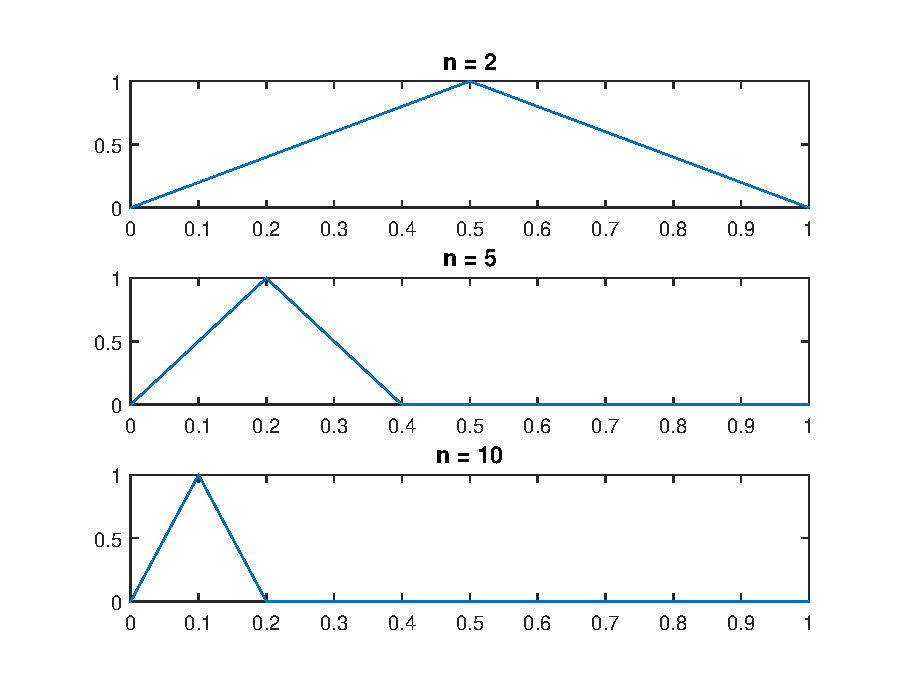
\includegraphics[width=1\textwidth]{../ex1/hatplot}
	\caption{Here we can see how the hat function behave for different values of n.}
	\label{fig:hatplot}
\end{figure}

To continue we have plotted the linear interpolant $\pi  f \in V_h$ of $f(x) = x(1-x)$ as defined by
\begin{equation}
	 \pi f(x) = \Sigma^n_{i=1} f(x_i) \phi_i(x)
	 \label{eq:inter}
\end{equation}
Which basically is just plotting the values of f(x) at certain points and dragging a straight line in between them. We illustrate this in figure \ref{fig:inter} for different amounts of points $n$. 
\begin{figure}[H]
	\centering
	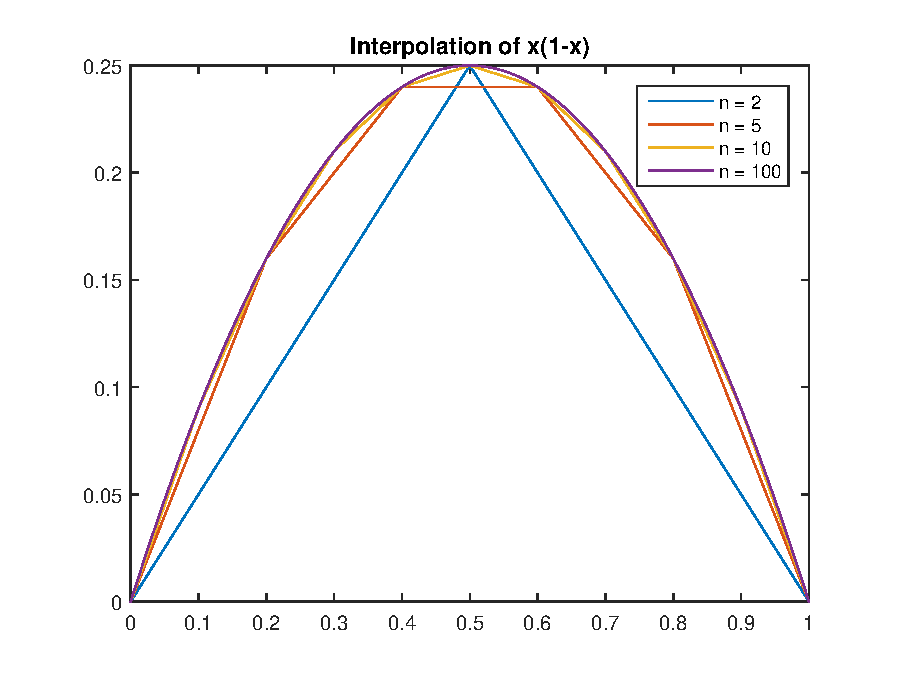
\includegraphics[width=1\textwidth]{../ex1/inter}
	\caption{An interpolation as described in equation \ref{eq:inter} for different values on $n$.}
	\label{fig:inter}
\end{figure}

In appendx \label{code:L2mass1D} we can see how the mass matrix for solving the $L^2$-projection problem was implemented. We use this mass matrix to calculate the $L^2$ projection $P_h f \in V_h$ of $f(x) = x(1-x)$. But to create the load vector for the problem we use two methods. The different values $b_i$ of the load vector $\bar{b}$ are basically 
\begin{equation}
	b_i = \int_{x_i - 1}^{x_i} f(\phi_i) dx + \int_{x_i}^{x_i+1} f(\phi_i) dx.
\end{equation}
In order to estimate these values we use either trapezoidal or simpsons method in this lab. The code for the code creating the load vector using the trapezoidal method is in appendix \ref{code:L2Load1D}, the code for the simpsons is in appendix \ref{code:LoadAssemblerS1D}. Looking at figure \ref{fig:l2proj} we can see how much better the values look like if one use the simpsons method to assemble the load vector compared to the trapezoidal. But one should not stop looking there. If we compare figure \ref{fig:inter} with figure \ref{fig:l2proj} we can see how the estimation methods differ. It is clear from figure \ref{fig:inter} that the first method we used tend to low ball the function value and if you where to integrate the estimation the value would come out consistently low\footnote{This would of course balance itself out if one where to do this estimation on say a sinus function that evenly goes up and down for infinity.}. Looking at figure \ref{fig:l2proj} we can instead see how the values goes over and under the correct values, thus given a more correct value, balanced around the correct one,  if one where to integrate the estimated function. This is natural since how the $L^2$ projection actually estimates the integral of the function. 
\begin{figure}[H]
	\centering
	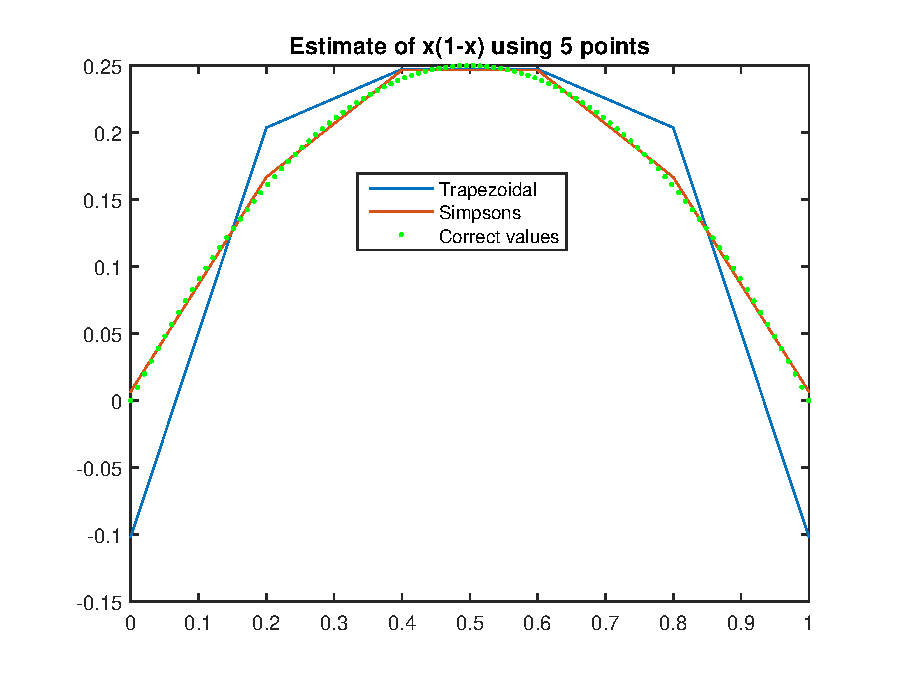
\includegraphics[width=1\textwidth]{../ex1/l2proj}
	\caption{Showing how the different approaches to the load vector assembly yeild different results.}
	\label{fig:l2proj}
\end{figure}

\newpage
\section{Problem 2}
\subsection{FEM Solution}
In this exersice we solve the initial value problem $-u'' = 2,0<x<1,u(0)=u(1)=0$. We use a uniform mesh with the step size $h = 1/2, 1/4, 1/16, 1/256$, between 0 and 1. The solution to this system, with the analytical solution, is depicted in figure \ref{fig:fem}
\begin{figure}[H]
	\centering
	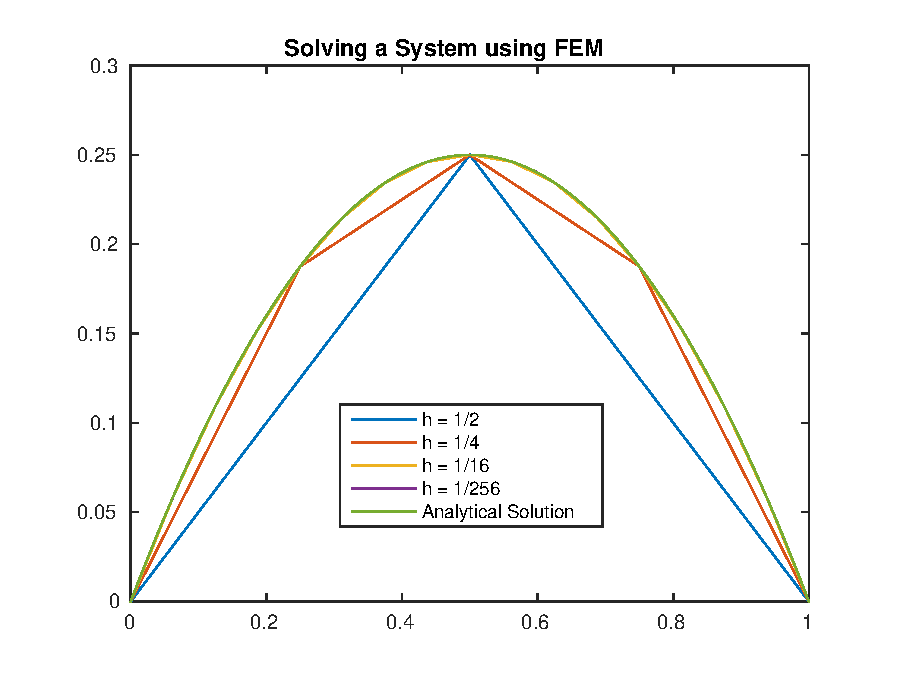
\includegraphics[width=1\textwidth]{../ex2/fem}
	\caption{A solution to the problem specified for the exercise, using FEM with different uniform mesh sizes.}
	\label{fig:fem}
\end{figure}

\subsection{Errror analysis}
In this exercise we only use priori error estimates. In order to look at the energy norm we want to prove that $||u - u_h||^2_E = ||u'||^2 - ||{u'}_h||^2$. 
\begin{align}
	||u-u_h||^2_E &= \int_I (u-u_h)'(u-u_h)dx = \int_I (u-u_h)'(u+u_h-u_h-u_h)'dx \\
	&= \int_I (u-u_h)'(u+u_h)'dx -  \int(u-u_h)'(u_h+u_h)'dx \\
	&= \int_I (u-u_h)'(u+u_h)'dx = \int_I ({u'}^2 - {u'}^2_h)dx =  ||u'||^2 - ||{u'}_h||^2 
\end{align}
where we use Galerkin orthogonality in the step from (4) to (5). From there we can just use the definition of the $L^2$ norm and $u_h$ to calculate the energy error. Calculating the $L^2$ error norm is done through taking $||P_hu - u_h||^2_{L^2(I)}$ as it is defined in the course book. Using this logic we end up with the expressions
\begin{align}
	||u - u_h||^2_E &= ||u'||^2_{L^2} - \bar{\xi}^T \bar{\bar{A}} \bar{\xi} \\
	&= 1/3 - \bar{\xi}^T \bar{\bar{A}} \bar{\xi}
\end{align}
\begin{align}
	||P_hu - u_h||^2_{L^2} = (\xi_{P_h} - \xi)' \bar{\bar{M}} (\xi_{P_h} - \xi)
\end{align}
where $\bar{\bar{A}}$ is the stiffness matrix, $\bar{\bar{M}}$ is the mass matrix, $\xi$ is the solution of the FEM system of equation, and $\xi_{P_h}$ is the solution to the $L^2$ projection problem.  The resulting log log plot of the error for different values of h is depicted in figure \ref{fig:loglogError}
\begin{figure}[H]
	\centering
	\includegraphics[width=1\textwidth]{../ex2/loglogError}
	\caption{The log log of different error norms at different mesh sizes.}
	\label{fig:loglogError}
\end{figure}
Already from the plot in figure \ref{fig:loglogError} we start to suspect that the dependence on h is stronger for the $L^2$ and maximum error norms. But this could easily be proven using table \ref{table:errors}. 
\begin{table}[H]
	\center
	\begin{tabular}{l | c c c c}
		norm/h & 1/2 & 1/4 & 1/16 & 1/256 \\
		\hline 
		Energy norm & $ 0.29$ & 0.14 & $3.6\cdot10^{-2}$ & $1.7\cdot10^{-3}$ \\
		$L^2$ norm & $4.1\cdot10^{-2}$ & $1.0\cdot10^{-3}$ & $6.5\cdot10^{-4}$ & $1.5\cdot10^{-6}$ \\
		Max norm & $6.2\cdot10^{-2}$ & $1.6\cdot10^{-2}$ & $9.7\cdot 10^{-4}$ & $2.8\cdot10^{-6}$
	\end{tabular}
	\caption{A table of all the error norms for the cases we tested.}
	\label{table:errors}
\end{table}
In the course book we can see equation 2.30 stating\footnote{The equation notation has been slightly rewritten}
\begin{equation}
	|| u - u_h ||^2_E \leq c h^1 ||u''||_{L^2}
\end{equation}
Making a system of two equations and using the values of the energy norm found at $h = 1/16$ and $h = 1/256$ we can solve to what exponential we have a dependence on h. The result is as expected that we have a value higher or equal to 1 in the exponential for h in the energy error norm, while we have a value higher or equal to two for the $L^2$ and maximum norm. 

\section{Problem 3}
In this exercise we implement a FEM solver that can deal with inhomogeneous boundary conditions. It is implemented based on the code presented in the course book under "2.3 A Model Problem with Variable Coefficients". Its slightly simplified though. The solution is presented in figure \ref{fig:inhom} and it was surprising how relatively simple it was to implement. 
\begin{figure}[H]
	\centering
	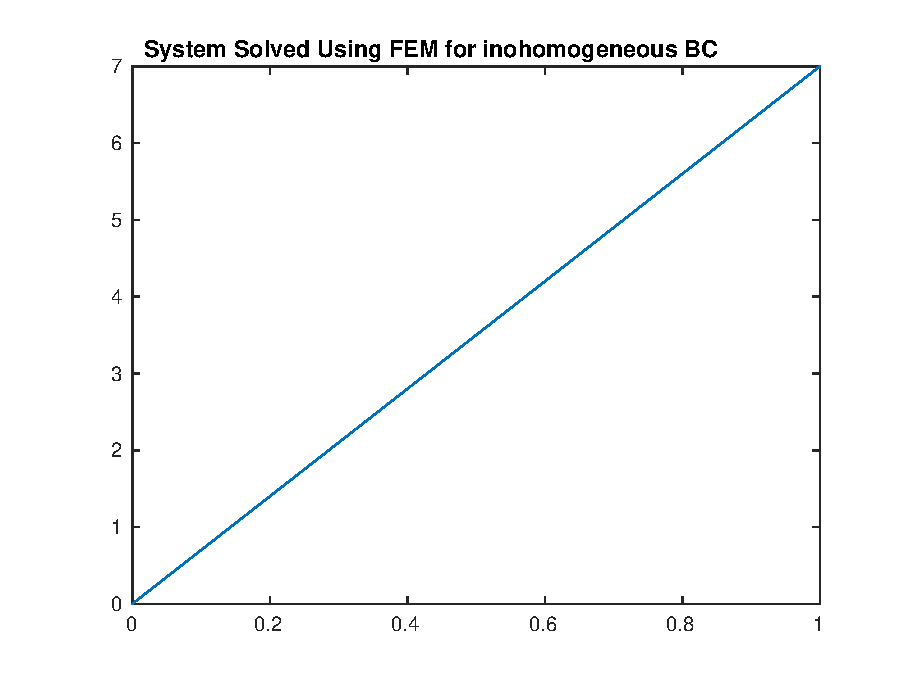
\includegraphics[width=1\textwidth]{../ex3/inhom}
	\caption{A fem solved using inhomogeneous boundary conditions}
	\label{fig:inhom}
\end{figure}


\newpage
\appendix
\section{Code for Problem 1}
\subsection{hatfun}\label{code:hatfun}
\verbatimtabinput{../ex1/hatfun.m}

\subsection{L2Mass1D}\label{code:L2Mass1D}
\verbatimtabinput{../ex1/L2Mass1D.m}

\subsection{L2Load1D}\label{code:L2Load1D}
\verbatimtabinput{../ex1/L2Load1D.m}

\subsection{LoadAssemblerS1D}\label{code:LoadAssemblerS1D}
\verbatimtabinput{../ex1/LoadAssemblerS1D.m}

\section{Code for Problem 2}
\subsection{solve}\label{code:solve}
\verbatimtabinput{../ex2/solve.m}

\subsection{LoadAssemblerS1D}\label{code:LoadAssemblerS1D}
\verbatimtabinput{../ex2/LoadAssemblerS1D.m}

\subsection{loadAssembly}\label{code:loadAssembly}
\verbatimtabinput{../ex2/loadAssembly.m}

\subsection{stiffAssembly}\label{code:stiffAssembly}
\verbatimtabinput{../ex2/stiffAssembly.m}

\subsection{L2Mass}\label{code:L2Mass1D}
\verbatimtabinput{../ex2/L2Mass1D.m}

\section{Code for Problem 3}
\subsection{solve}\label{code:solve}
\verbatimtabinput{../ex3/solve.m}

\subsection{LoadAssemblerS1D}\label{code:LoadAssemblerS1D}
\verbatimtabinput{../ex3/LoadAssemblerS1D.m}

\subsection{sourceAssembler1D}\label{code:sourceAssembler1D}
\verbatimtabinput{../ex3/sourceAssembler1D.m}

\subsection{stiffnessAssembler1D}\label{code:stiffnessAssembler1D}
\verbatimtabinput{../ex2/stiffnessAssembler1D.m}

\end{document}
